% !TEX root = ../main.tex
% =============================================================================
% CHAPTER 5 - EXPERIMENTS & RESULTS
% VOICE: impersonal passive. Never "we", never "I". See ../STYLE_GUIDE.md.
% Tense: past for what was measured; present for what a table shows.
% =============================================================================

\chapter{Results}\label{ch:results}

This chapter evaluates not only whether the learned EEG representations support
clinical classification, but also the conditions under which that information
remains useful. The analysis therefore proceeds from within-dataset
five-fold cross-validation to leave-one-subject-out (LOSO) evaluation and then
to cross-dataset transfer from FEP to SCZ. This progression separates
performance on unseen participants from robustness to a change of dataset.
The remaining experiments examine how the representations are used and where
task relevant information is expressed, through finetuning, masking ablations,
layer-wise analysis, the CLS perturbation experiment, and
classification using reconstructed EEG. Unless otherwise stated, all
downstream metrics are reported at the participant level using the procedures
defined in Section~\ref{sec:m_protocols}.


\section{How to Read the Results}\label{sec:r_reading}

Three points are important when interpreting the results in this chapter.

First, balanced accuracy (BAcc) and area under the precision-recall curve
(AUPRC) were both calculated at the participant level, but by different forms of
aggregation: BAcc from the majority vote label and AUPRC from the mean patient
class probability (Section~\ref{sec:m_metrics}). They therefore need not change
in the same direction. A model may rank participants well by their mean
probabilities while still assigning some of them to the wrong class at the
decision threshold.

\begin{table}[htbp]
  \centering
  \small
  \caption[Chance reference levels by task]{Downstream cohort sizes and chance levels of the two reported metrics.}
  \label{tab:chance_levels}
  \begin{tabular}{l c c c c}
    \toprule
    Task & Subjects & Patients / HC & AUPRC chance & BAcc chance \\
    \midrule
    AD versus HC   & 52 & 29 / 23 & 55.8 & 50.0 \\
    FTD versus HC  & 41 & 18 / 23 & 43.9 & 50.0 \\
    FEP versus HC  & 62 & 38 / 24 & 61.3 & 50.0 \\
    MDD versus HC  & 98 & 26 / 72 & 26.5 & 50.0 \\
    \midrule
    SCZ (external test) & 77 & 30 / 47 & 39.0 & 50.0 \\
    \bottomrule
  \end{tabular}
  \\[3pt]
  \begin{minipage}{0.92\linewidth}\footnotesize\raggedright
    Subject counts are the downstream evaluation pools remaining after the pretraining reserve participants were removed (Section~\ref{sec:m_datasets}). The SCZ cohort was never used for training and appears only as the external test set in Section~\ref{sec:r_crossdataset}.
  \end{minipage}
\end{table}

Second, AUPRC was computed using average precision with the patient group as
the positive class (Section~\ref{sec:m_metrics}). Its prevalence reference
therefore differs across tasks. Table~\ref{tab:chance_levels} lists the
downstream cohort sizes currently reported in the study and the corresponding
reference levels. For example, the reference AUPRC is 26.5\% for MDD and
61.3\% for FEP. BAcc has a nominal chance level of 50\% for each binary task.
Accordingly, AUPRC comparisons in this chapter are made primarily between
models evaluated on the same task. BAcc has a common nominal chance level, but
comparisons across tasks should still be interpreted cautiously because the
datasets and classification problems differ.

Third, no inferential significance tests were performed for comparisons among
the downstream models, so these comparisons are descriptive. For the
five-fold results, the reported standard deviation describes variation across
the five folds rather than statistical uncertainty about a population effect.
For LOSO, predictions were pooled across test participants to produce one BAcc
and one AUPRC value, so no fold level standard deviation is available
(Section~\ref{sec:m_loso}). Bold and underlined values in the result tables
mark only the highest and second-highest numerical values and should not be
interpreted as evidence of statistically significant differences.


\section{Within-Dataset Performance}\label{sec:r_indomain}

\begin{table}[htbp]
  \centering
  \small
  \setlength{\tabcolsep}{3pt}
  \caption[Within-dataset classification performance]{In-domain classification performance on four clinical EEG tasks (subject level, mean\,$\pm$\,std over five-fold cross-validation).}
  \label{tab:indomain}
  \resizebox{\ifdim\width>\linewidth\linewidth\else\width\fi}{!}{%
  \begin{tabular}{l cc cc cc cc}
    \toprule
     & \multicolumn{2}{c}{AD} & \multicolumn{2}{c}{FTD} & \multicolumn{2}{c}{FEP} & \multicolumn{2}{c}{MDD} \\
    \cmidrule(lr){2-3} \cmidrule(lr){4-5} \cmidrule(lr){6-7} \cmidrule(lr){8-9}
     & AUPRC $\uparrow$ & BAcc $\uparrow$ & AUPRC $\uparrow$ & BAcc $\uparrow$ & AUPRC $\uparrow$ & BAcc $\uparrow$ & AUPRC $\uparrow$ & BAcc $\uparrow$ \\
    \midrule
    LDA & 95.0\,{\scriptsize$\pm$5.4} & \underline{87.3\,{\scriptsize$\pm$10.6}} & 82.0\,{\scriptsize$\pm$12.6} & 77.5\,{\scriptsize$\pm$13.3} & 72.3\,{\scriptsize$\pm$2.5} & 57.9\,{\scriptsize$\pm$7.2} & 35.3\,{\scriptsize$\pm$11.8} & 49.4\,{\scriptsize$\pm$11.5} \\
    SVM & 93.0\,{\scriptsize$\pm$7.0} & 80.8\,{\scriptsize$\pm$11.0} & 82.1\,{\scriptsize$\pm$13.3} & 66.3\,{\scriptsize$\pm$23.6} & 75.4\,{\scriptsize$\pm$14.3} & 56.8\,{\scriptsize$\pm$19.4} & 38.7\,{\scriptsize$\pm$13.2} & \underline{55.0\,{\scriptsize$\pm$10.8}} \\
    XGBoost & 95.4\,{\scriptsize$\pm$5.3} & 85.3\,{\scriptsize$\pm$11.1} & 79.3\,{\scriptsize$\pm$16.0} & 68.3\,{\scriptsize$\pm$14.1} & 70.4\,{\scriptsize$\pm$11.1} & 51.1\,{\scriptsize$\pm$10.3} & 33.8\,{\scriptsize$\pm$11.6} & 54.9\,{\scriptsize$\pm$6.8} \\
    \midrule
    EEGNeX & 95.3\,{\scriptsize$\pm$4.8} & 80.8\,{\scriptsize$\pm$17.4} & \underline{89.8\,{\scriptsize$\pm$15.6}} & \textbf{81.3\,{\scriptsize$\pm$15.7}} & 67.9\,{\scriptsize$\pm$12.3} & 52.5\,{\scriptsize$\pm$13.6} & 40.8\,{\scriptsize$\pm$14.1} & 50.0\,{\scriptsize$\pm$0.0} \\
    EEGConformer & 94.3\,{\scriptsize$\pm$3.3} & 67.8\,{\scriptsize$\pm$10.9} & 83.5\,{\scriptsize$\pm$7.7} & 64.2\,{\scriptsize$\pm$13.8} & 73.1\,{\scriptsize$\pm$6.9} & 53.2\,{\scriptsize$\pm$9.0} & \underline{45.7\,{\scriptsize$\pm$22.1}} & 50.3\,{\scriptsize$\pm$0.6} \\
    ATCNet & 93.7\,{\scriptsize$\pm$6.8} & 85.3\,{\scriptsize$\pm$13.7} & 86.2\,{\scriptsize$\pm$14.2} & 79.2\,{\scriptsize$\pm$10.5} & 77.1\,{\scriptsize$\pm$7.3} & \textbf{60.4\,{\scriptsize$\pm$7.8}} & \textbf{46.0\,{\scriptsize$\pm$17.5}} & 48.0\,{\scriptsize$\pm$4.0} \\
    \midrule
    LaBraM (LP) & 89.9\,{\scriptsize$\pm$11.2} & 73.5\,{\scriptsize$\pm$18.2} & 69.5\,{\scriptsize$\pm$21.5} & 73.5\,{\scriptsize$\pm$19.0} & 68.2\,{\scriptsize$\pm$5.5} & 51.5\,{\scriptsize$\pm$8.9} & 36.4\,{\scriptsize$\pm$6.9} & 50.0\,{\scriptsize$\pm$0.0} \\
    CBraMod (LP) & 92.1\,{\scriptsize$\pm$6.6} & 80.0\,{\scriptsize$\pm$7.8} & 75.8\,{\scriptsize$\pm$18.7} & 68.0\,{\scriptsize$\pm$14.8} & 68.1\,{\scriptsize$\pm$3.5} & 47.1\,{\scriptsize$\pm$7.1} & 28.5\,{\scriptsize$\pm$7.4} & 49.3\,{\scriptsize$\pm$1.3} \\
    REVE (LP) & \underline{97.1\,{\scriptsize$\pm$2.5}} & 81.7\,{\scriptsize$\pm$12.0} & \textbf{91.3\,{\scriptsize$\pm$9.0}} & \underline{80.5\,{\scriptsize$\pm$12.0}} & \textbf{81.0\,{\scriptsize$\pm$4.8}} & \underline{58.5\,{\scriptsize$\pm$3.2}} & 33.3\,{\scriptsize$\pm$10.2} & 52.9\,{\scriptsize$\pm$3.9} \\
    \midrule
    BrainLM-EEG (LP) & 95.9\,{\scriptsize$\pm$5.7} & 78.8\,{\scriptsize$\pm$15.6} & 83.8\,{\scriptsize$\pm$16.3} & 69.2\,{\scriptsize$\pm$15.9} & 77.0\,{\scriptsize$\pm$6.0} & 56.5\,{\scriptsize$\pm$9.7} & 30.4\,{\scriptsize$\pm$7.9} & 52.6\,{\scriptsize$\pm$5.1} \\
    BrainLM-EEG-RoPE (LP) & 92.4\,{\scriptsize$\pm$6.7} & 81.2\,{\scriptsize$\pm$13.3} & 73.0\,{\scriptsize$\pm$16.3} & 48.5\,{\scriptsize$\pm$15.2} & 74.6\,{\scriptsize$\pm$4.5} & 52.8\,{\scriptsize$\pm$12.0} & 36.3\,{\scriptsize$\pm$12.8} & 50.0\,{\scriptsize$\pm$0.0} \\
    BrainLM-EEG-Microstate (LP) & \textbf{100.0\,{\scriptsize$\pm$0.0}} & \textbf{87.3\,{\scriptsize$\pm$8.9}} & 87.0\,{\scriptsize$\pm$14.5} & 76.3\,{\scriptsize$\pm$12.7} & \underline{80.5\,{\scriptsize$\pm$5.1}} & 54.5\,{\scriptsize$\pm$6.3} & 32.5\,{\scriptsize$\pm$12.2} & \textbf{55.3\,{\scriptsize$\pm$6.8}} \\
    \bottomrule
  \end{tabular}%
  }
  \\[3pt]
  \begin{minipage}{\linewidth}\footnotesize\raggedright
    AD: Alzheimer's disease; FTD: frontotemporal dementia; FEP: first-episode psychosis; MDD: major depressive disorder; all versus healthy controls. LP: linear probe. Values are subject level $\times 100$. \textbf{Bold}: best per column; \underline{underline}: second best.
  \end{minipage}
\end{table}


Table~\ref{tab:indomain} reports performance under the five-fold
within-dataset protocol described in Section~\ref{sec:m_fivefold}. The first
pattern is task dependence: performance differed substantially across the four
clinical tasks, and the model ordering also changed from one task to another.
The results are therefore interpreted first within each task rather than as a
single overall ranking of model families.

For AD versus HC, all model families achieved an AUPRC of at least 89.9\%,
compared with an AUPRC reference of 55.8\%. BAcc ranged from 67.8\% for
EEGConformer to 87.3\% for BrainLM-EEG-Microstate and LDA, which both
reported the highest BAcc, while the Microstate variant also achieved 100\%
AUPRC. These values are not contradictory because AUPRC was calculated from
mean participant level probabilities, whereas BAcc used majority vote class
predictions (Section~\ref{sec:r_reading}). This AUPRC therefore indicates perfect ranking within the evaluated folds, not
perfect classification at the decision threshold. Because both the proposed models and the comparison
baselines performed strongly, these results do not provide evidence of a
specific advantage for self-supervised pretraining on this task
(Figure~\ref{fig:indomain_overview}).

% Generated by code/analysis/dataset/generate_results_figures.py, which writes
% the PDF directly into manuscript/figures/. Authored at \textwidth (6.20 in)
% so the include applies no scaling. Do not resize here.
\begin{figure}[htbp]
\centering
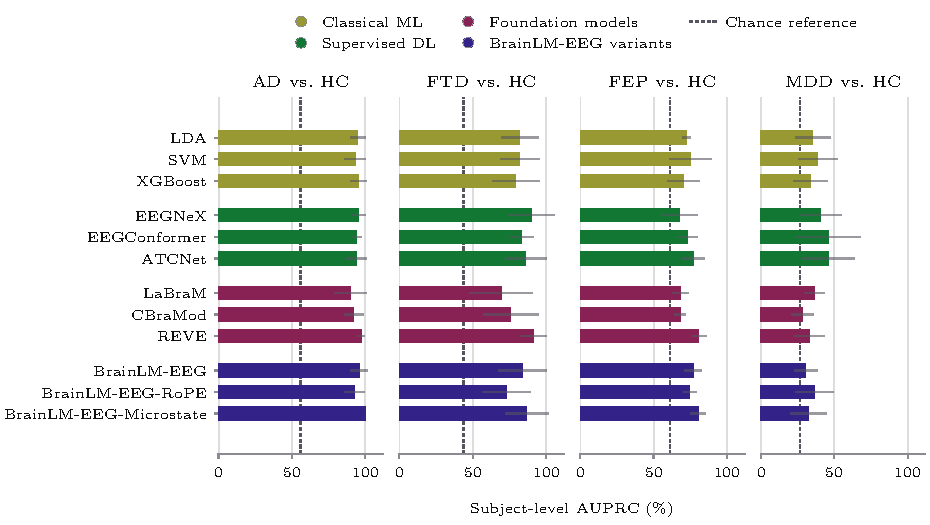
\includegraphics[width=\textwidth]{figures/fig_indomain_overview.pdf}
\caption[Within-dataset AUPRC by model and task]{
Subject level AUPRC for each task. Bars are grouped by model family; error bars
denote fold standard deviation, and dashed lines indicate the task specific
AUPRC chance reference.
}
\label{fig:indomain_overview}
\end{figure}

For FTD versus HC, EEGNeX and REVE achieved the highest BAcc values, at 81.3\%
and 80.5\%, respectively. BrainLM-EEG-RoPE achieved 48.5\% BAcc, below the
nominal 50\% chance level. The model ordering changed under LOSO, as reported
in Section~\ref{sec:r_loso}. For FEP versus HC, REVE reported the highest
AUPRC at 81.0\%, followed by BrainLM-EEG-Microstate at 80.5\%. ATCNet reported
the highest BAcc at 60.4\%, and CBraMod reported the lowest at 47.1\%. The
highest FEP AUPRC was therefore 19.7
percentage points above the 61.3\% prevalence reference for this task.

For MDD versus HC, ATCNet and EEGConformer achieved AUPRC values of 46.0\% and
45.7\%, respectively, above the 26.5\% prevalence reference. In contrast, BAcc
ranged from 48.0\% to 55.3\% across models. Several models had BAcc values very
close to 50\%, including values of exactly 50.0\% for EEGNeX, LaBraM, and
BrainLM-EEG-RoPE. Overall, some models showed above-reference ranking on MDD,
whereas thresholded participant level classification remained close to chance.
These results do not determine whether this pattern reflects the dataset, the
learned representations, the classification heads, or the chosen decision
rule.

The within-dataset results establish a task-dependent baseline. AD was strongly decodable across model families, whereas the relative model ordering was less stable on FTD and FEP, and MDD showed a clearer separation between ranking performance and thresholded classification. Within the BrainLM-EEG family, the Microstate variant achieved higher numerical performance than the base model in several task metric comparisons, whereas the RoPE variant showed a less consistent pattern. However, neither modification was consistently better across tasks or metrics, and the observed fold-to-fold variation further limits the interpretation of small numerical differences. The next analysis therefore examines whether these patterns remain when each participant receives an out-of-sample prediction under LOSO.



\section{Leave-One-Subject-Out Evaluation}\label{sec:r_loso}

\begin{table}[htbp]
  \centering
  \small
  \setlength{\tabcolsep}{3pt}
  \caption[Leave-one-subject-out evaluation]{Leave-one-subject-out (LOSO) evaluation on four clinical EEG tasks.}
  \label{tab:loso}
  \resizebox{\ifdim\width>\linewidth\linewidth\else\width\fi}{!}{%
  \begin{tabular}{l cc cc cc cc}
    \toprule
     & \multicolumn{2}{c}{AD} & \multicolumn{2}{c}{FTD} & \multicolumn{2}{c}{FEP} & \multicolumn{2}{c}{MDD} \\
    \cmidrule(lr){2-3} \cmidrule(lr){4-5} \cmidrule(lr){6-7} \cmidrule(lr){8-9}
     & AUPRC $\uparrow$ & BAcc $\uparrow$ & AUPRC $\uparrow$ & BAcc $\uparrow$ & AUPRC $\uparrow$ & BAcc $\uparrow$ & AUPRC $\uparrow$ & BAcc $\uparrow$ \\
    \midrule
    LDA & 92.2 & 85.8 & 85.0 & 78.4 & \textbf{78.9} & \underline{66.0} & 34.2 & 57.2 \\
    SVM & 93.4 & 85.3 & 75.8 & 71.3 & 65.6 & 55.8 & 30.7 & 50.5 \\
    XGBoost & 94.9 & 82.7 & 77.1 & 62.9 & 67.0 & 59.5 & 38.6 & 55.1 \\
    \midrule
    EEGNeX & 92.9 & 83.1 & 86.9 & 80.2 & 63.1 & 50.5 & \underline{41.9} & 54.1 \\
    EEGConformer & 96.8 & 86.6 & \underline{95.0} & 77.8 & 60.7 & 44.1 & 34.7 & \underline{58.8} \\
    ATCNet & 92.8 & \underline{87.0} & 89.2 & 79.0 & \textbf{78.9} & \textbf{68.4} & 37.4 & 54.6 \\
    \midrule
    LaBraM (LP) & 93.1 & 85.3 & 88.7 & 79.6 & 54.4 & 43.9 & \textbf{42.5} & 53.2 \\
    CBraMod (LP) & 95.9 & 85.7 & 80.9 & 75.2 & 56.5 & 43.3 & 34.4 & 50.5 \\
    REVE (LP) & \textbf{98.0} & \textbf{90.9} & \textbf{95.5} & 91.7 & 62.2 & 45.4 & 37.7 & \textbf{61.4} \\
    \midrule
    BrainLM-EEG (LP) & 94.7 & 81.4 & 86.2 & 81.8 & 68.3 & 61.1 & 32.9 & 49.5 \\
    BrainLM-EEG-RoPE (LP) & 96.1 & \underline{87.0} & 92.3 & \textbf{92.9} & \underline{68.7} & 43.9 & 36.3 & 51.1 \\
    BrainLM-EEG-Microstate (LP) & \underline{96.9} & 85.3 & 94.6 & \underline{92.3} & 62.8 & 56.9 & 37.9 & 51.6 \\
    \bottomrule
  \end{tabular}%
  }
  \\[3pt]
  \begin{minipage}{\linewidth}\footnotesize\raggedright
    AD: Alzheimer's disease; FTD: frontotemporal dementia; FEP: first-episode psychosis; MDD: major depressive disorder; all versus healthy controls. LP: linear probe. Values are subject level $\times 100$. \textbf{Bold}: best per column; \underline{underline}: second best.
  \end{minipage}
\end{table}


The LOSO procedure is described in Section~\ref{sec:m_loso}. Each iteration used one participant for testing, one for validation, and the remaining participants for training. After every participant had served as the test participant once, the out-of-sample predictions were pooled to calculate a single BAcc and AUPRC value for each model and task. Table~\ref{tab:loso} reports these results. Because each LOSO test fold contains only one participant, BAcc and AUPRC cannot be meaningfully calculated at the fold level, in particular balanced accuracy requires observations from both classes. The metrics were therefore calculated once from the pooled out-of-sample predictions.


For AD versus HC, all model families again achieved relatively high
performance. REVE had the highest values, with 98.0\% AUPRC and 90.9\% BAcc,
while several other models, including the BrainLM-EEG variants, were within a
few percentage points. For FTD versus HC, the strongest numerical results
depended on the metric. REVE achieved the highest AUPRC at 95.5\%, followed by
EEGConformer at 95.0\% and BrainLM-EEG-Microstate at 94.6\%. For BAcc,
BrainLM-EEG-RoPE and BrainLM-EEG-Microstate achieved 92.9\% and 92.3\%,
respectively, compared with 91.7\% for REVE.

For FEP versus HC, several pretrained models achieved lower AUPRC values under
LOSO than under five-fold evaluation. ATCNet and LDA each achieved 78.9\%
AUPRC, while a number of self-supervised and pretrained foundation models reported
lower values. For MDD, AUPRC ranged from 30.7\% to 42.5\%, with LaBraM
highest at 42.5\% and EEGNeX second at 41.9\%, whereas BAcc ranged from 49.5\%
to 61.4\%, with multiple models remaining close to the nominal 50\% chance
level.

Within the proposed model family, both RoPE and Microstate achieved higher numerical AUPRC and BAcc than the base BrainLM-EEG model on AD and FTD. The same pattern was not observed consistently for FEP or MDD, indicating that the relative benefit of the proposed modifications was task dependent.


A particularly large protocol-dependent change occurred for FTD. BrainLM-EEG-RoPE
changed from 73.0\% AUPRC and 48.5\% BAcc under five-fold cross-validation to
92.3\% AUPRC and 92.9\% BAcc under LOSO. BrainLM-EEG-Microstate changed from
87.0\% AUPRC and 76.3\% BAcc to 94.6\% AUPRC and 92.3\% BAcc. Because the FTD
evaluation pool contained only 41 participants, the individual five-fold test
sets were small. The marked difference between protocols therefore indicates
that the reported performance and model ordering were sensitive to the
resampling scheme in this dataset. Pooling the LOSO predictions removes
fold-to-fold reporting variation, but it does not remove uncertainty associated
with the small cohort.

% Generated by code/analysis/dataset/generate_results_figures.py.
\begin{figure}[htbp]
\centering
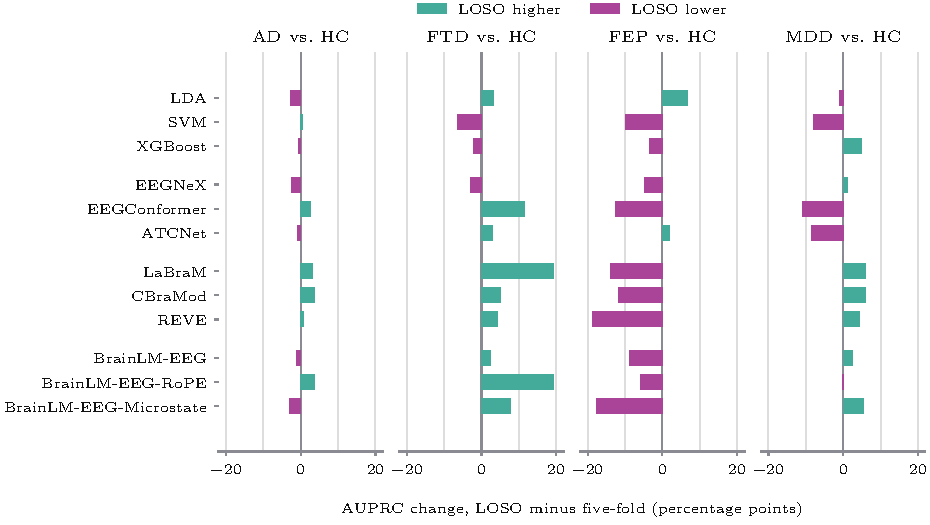
\includegraphics[width=\textwidth]{figures/fig_loso_vs_5fold.pdf}
\caption[Five-fold versus LOSO AUPRC]{
Difference in subject level AUPRC between pooled LOSO and five-fold cross-validation
for each model and task. Bars show LOSO minus five-fold AUPRC.
}
\label{fig:loso_vs_5fold}
\end{figure}

Changes between protocols did not consistently favour the proposed models. On
FEP, REVE changed from 81.0\% AUPRC under five-fold evaluation to 62.2\% under
LOSO, while LaBraM changed from 68.2\% to 54.4\%. Under LOSO, LDA achieved a
higher FEP AUPRC than the evaluated foundation models. For some model task
combinations, the differences between evaluation protocols were therefore as
large as or larger than the numerical differences between model families.
Figure~\ref{fig:loso_vs_5fold} shows the protocol difference for every model and
task.

The LOSO analysis therefore reinforces the sensitivity of the reported model comparisons to the evaluation protocol. The BrainLM-EEG variants were among the stronger models on FTD when predictions from all held-out participants were pooled, demonstrating that the pretrained representations supported strong participant level decoding on this task. At these cohort sizes, which model appears to perform best can depend on which participants are included in the training and test sets.


\section{Cross-Dataset Generalisation from FEP to SCZ}\label{sec:r_crossdataset}

\begin{table}[htbp]
  \centering
  \small
  \setlength{\tabcolsep}{3pt}
  \caption[Cross-dataset transfer from FEP to SCZ]{Cross-dataset transfer from FEP to SCZ, alongside in-domain FEP performance (subject level).}
  \label{tab:cross_eval}
  \resizebox{\ifdim\width>\linewidth\linewidth\else\width\fi}{!}{%
  \begin{tabular}{l cc cc cc}
    \toprule
     & \multicolumn{2}{c}{FEP} & \multicolumn{2}{c}{FEP $\to$ SCZ (five-fold)} & \multicolumn{2}{c}{FEP $\to$ SCZ (all-data)} \\
    \cmidrule(lr){2-3} \cmidrule(lr){4-5} \cmidrule(lr){6-7}
     & AUPRC $\uparrow$ & BAcc $\uparrow$ & AUPRC $\uparrow$ & BAcc $\uparrow$ & AUPRC $\uparrow$ & BAcc $\uparrow$ \\
    \midrule
    LDA & 72.3\,{\scriptsize$\pm$2.5} & 57.9\,{\scriptsize$\pm$7.2} & 40.2\,{\scriptsize$\pm$4.0} & 50.0\,{\scriptsize$\pm$3.6} & 39.2 & 55.2 \\
    SVM & 75.4\,{\scriptsize$\pm$14.3} & 56.8\,{\scriptsize$\pm$19.4} & 43.2\,{\scriptsize$\pm$4.8} & 53.8\,{\scriptsize$\pm$2.7} & 54.4 & 55.3 \\
    XGBoost & 70.4\,{\scriptsize$\pm$11.1} & 51.1\,{\scriptsize$\pm$10.3} & 42.4\,{\scriptsize$\pm$3.0} & 47.4\,{\scriptsize$\pm$2.2} & 41.8 & 51.4 \\
    \midrule
    EEGNeX & 67.9\,{\scriptsize$\pm$12.3} & 52.5\,{\scriptsize$\pm$13.6} & 43.3\,{\scriptsize$\pm$8.7} & 50.8\,{\scriptsize$\pm$2.9} & \textbf{57.6} & \textbf{63.4} \\
    EEGConformer & 73.1\,{\scriptsize$\pm$6.9} & 53.2\,{\scriptsize$\pm$9.0} & 47.2\,{\scriptsize$\pm$2.3} & 51.7\,{\scriptsize$\pm$2.2} & 48.4 & 55.7 \\
    ATCNet & 77.1\,{\scriptsize$\pm$7.3} & \textbf{60.4\,{\scriptsize$\pm$7.8}} & \textbf{54.4\,{\scriptsize$\pm$6.9}} & \underline{56.5\,{\scriptsize$\pm$3.9}} & 49.5 & \underline{62.7} \\
    \midrule
    LaBraM (LP) & 68.2\,{\scriptsize$\pm$5.5} & 51.5\,{\scriptsize$\pm$8.9} & 48.5\,{\scriptsize$\pm$4.8} & 51.3\,{\scriptsize$\pm$3.4} & \underline{56.8} & 57.6 \\
    CBraMod (LP) & 68.1\,{\scriptsize$\pm$3.5} & 47.1\,{\scriptsize$\pm$7.1} & 43.0\,{\scriptsize$\pm$6.7} & 50.2\,{\scriptsize$\pm$3.3} & 42.9 & 51.5 \\
    REVE (LP) & \textbf{81.0\,{\scriptsize$\pm$4.8}} & \underline{58.5\,{\scriptsize$\pm$3.2}} & 46.1\,{\scriptsize$\pm$5.5} & 55.8\,{\scriptsize$\pm$3.0} & 45.2 & 57.6 \\
    \midrule
    BrainLM-EEG (LP) & 77.0\,{\scriptsize$\pm$6.0} & 56.5\,{\scriptsize$\pm$9.7} & 50.5\,{\scriptsize$\pm$5.8} & 52.3\,{\scriptsize$\pm$2.4} & 42.2 & 56.1 \\
    BrainLM-EEG-RoPE (LP) & 74.6\,{\scriptsize$\pm$4.5} & 52.8\,{\scriptsize$\pm$12.0} & 52.7\,{\scriptsize$\pm$4.7} & 55.7\,{\scriptsize$\pm$4.7} & 47.4 & 61.3 \\
    BrainLM-EEG-Microstate (LP) & \underline{80.5\,{\scriptsize$\pm$5.1}} & 54.5\,{\scriptsize$\pm$6.3} & \underline{53.1\,{\scriptsize$\pm$2.4}} & \textbf{58.1\,{\scriptsize$\pm$4.5}} & 46.2 & 49.5 \\
    \bottomrule
  \end{tabular}%
  }
  \\[3pt]
  \begin{minipage}{\linewidth}\footnotesize\raggedright
    FEP: first-episode psychosis; SCZ: schizophrenia; all versus healthy controls. LP: linear probe. Values are subject level $\times 100$. \textbf{Bold}: best per column; \underline{underline}: second best.
  \end{minipage}
\end{table}


Cross-dataset evaluation examined whether models developed on FEP transferred
to an independently collected SCZ cohort, following
Section~\ref{sec:m_crossdataset}. The two datasets were collected independently
and differed in cohort and acquisition characteristics
\parencite{deansalisburyEEGFirstEpisode2022,raczReducedTemporalVariability2025}.
The comparison therefore reflects a combined dataset and acquisition shift
rather than isolating any single source of distribution shift.

Table~\ref{tab:cross_eval} reports three settings. The first column gives
within-dataset FEP performance from five-fold cross-validation. In the second
setting, each of the five FEP-trained checkpoints was evaluated directly on
SCZ and the resulting metrics were averaged. In the third setting, a model
trained on the complete FEP data was evaluated once on SCZ.

% Generated by code/analysis/dataset/generate_results_figures.py.
\begin{figure}[htbp]
\centering
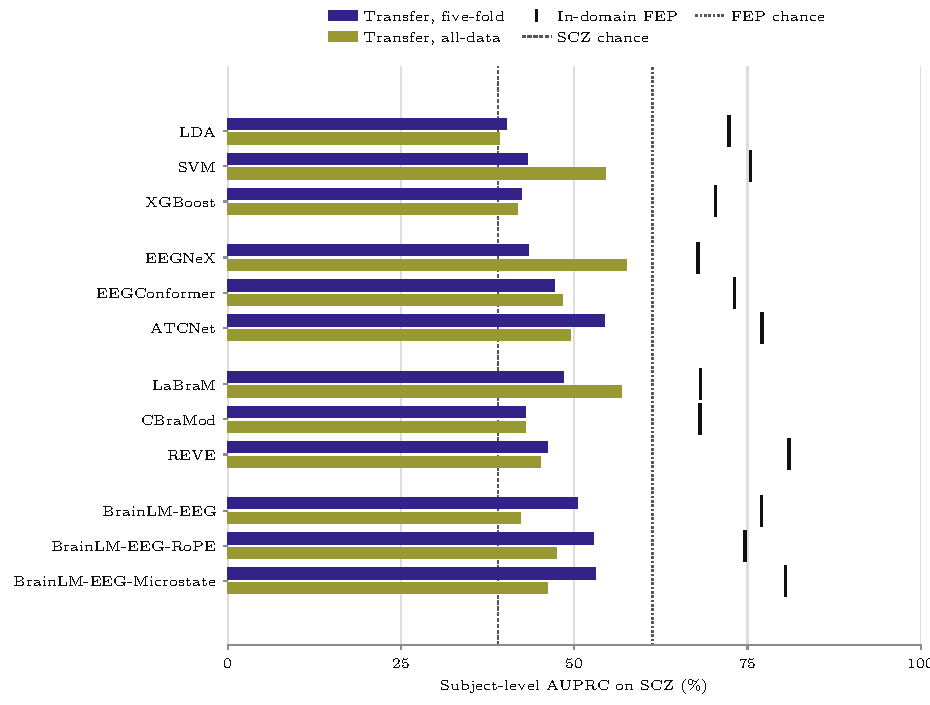
\includegraphics[width=\textwidth]{figures/fig_transfer_overview.pdf}
\caption[FEP-to-SCZ transfer AUPRC]{
Subject level AUPRC on SCZ for five-fold and all-data FEP transfer checkpoints.
Vertical rules indicate each model's in-domain FEP AUPRC; dashed and dotted lines
denote the SCZ and FEP chance references, respectively.
}
\label{fig:transfer_overview}
\end{figure}

AUPRC decreased for every model when the FEP-trained models were evaluated on
SCZ under either transfer setting. In the five-checkpoint setting, ATCNet
achieved the highest AUPRC at 54.4\%, followed by BrainLM-EEG-Microstate at
53.1\% and BrainLM-EEG-RoPE at 52.7\%, while LDA achieved the lowest AUPRC of 40.2\%. The
externally pretrained models showed a similar reduction, with REVE, LaBraM, and
CBraMod achieving 46.1\%, 48.5\%, and 43.0\% AUPRC, respectively, in this
setting. In the
full-FEP training setting, EEGNeX achieved the highest AUPRC and BAcc, at
57.6\% and 63.4\%, respectively. Across the transfer results, BAcc ranged from
47.4\% to 63.4\%. Using the SCZ class counts currently reported in
Table~\ref{tab:chance_levels}, the AUPRC prevalence reference is 39.0\%.
Figure~\ref{fig:transfer_overview} places these transfer values beside each
model's in-domain FEP result.

Within the BrainLM-EEG family, both variants achieved higher AUPRC than the base model in both transfer settings, whereas the corresponding BAcc differences were not consistently positive. No model family showed a consistent numerical robustness advantage across the
two transfer settings. For example, EEGNeX changed from 43.3\% AUPRC in the
five-checkpoint setting to 57.6\% when trained on the full-FEP data, whereas BrainLM-EEG-Microstate changed from 53.1\% to 46.2\%. Because
the full-data setting is based on a single trained checkpoint, it provides no
estimate of run-to-run variation. Differences between the two transfer
settings should therefore be interpreted descriptively.

The FEP to SCZ experiment therefore establishes an important
boundary on the preceding within-dataset results. Models that produced
out-of-sample predictions for unseen participants from the source dataset did
not retain the same ranking performance after transfer to the external
dataset. The transfer was limited and variable across model families, and no
family showed a consistent robustness advantage across the two transfer
settings. This does not establish that the learned representations cannot
transfer across datasets more generally. Because FEP performance was itself
protocol dependent, the experiment also cannot separate the effect of dataset
shift from limitations of the source task model. A stronger assessment would
require additional external dataset pairs.


\section{Linear Probing versus Finetuning}\label{sec:r_finetune}

\begin{table}[htbp]
  \centering
  \small
  \setlength{\tabcolsep}{3pt}
  \caption[Linear probing versus full finetuning]{Linear probing versus full finetuning of BrainLM-EEG model variants under LOSO evaluation.}
  \label{tab:loso_ft}
  \resizebox{\ifdim\width>\linewidth\linewidth\else\width\fi}{!}{%
  \begin{tabular}{l cc cc cc cc}
    \toprule
     & \multicolumn{2}{c}{AD} & \multicolumn{2}{c}{FTD} & \multicolumn{2}{c}{FEP} & \multicolumn{2}{c}{MDD} \\
    \cmidrule(lr){2-3} \cmidrule(lr){4-5} \cmidrule(lr){6-7} \cmidrule(lr){8-9}
     & AUPRC $\uparrow$ & BAcc $\uparrow$ & AUPRC $\uparrow$ & BAcc $\uparrow$ & AUPRC $\uparrow$ & BAcc $\uparrow$ & AUPRC $\uparrow$ & BAcc $\uparrow$ \\
    \midrule
    BrainLM-EEG (LP) & 94.7 & 81.4 & 86.2 & 81.8 & \underline{68.3} & \textbf{61.1} & 32.9 & 49.5 \\
    BrainLM-EEG-RoPE (LP) & \underline{96.1} & \textbf{87.0} & \underline{92.3} & \textbf{92.9} & \textbf{68.7} & 43.9 & \underline{36.3} & 51.1 \\
    BrainLM-EEG-Microstate (LP) & \textbf{96.9} & \underline{85.3} & \textbf{94.6} & \underline{92.3} & 62.8 & \underline{56.9} & \textbf{37.9} & \underline{51.6} \\
    \midrule
    BrainLM-EEG (FT) & 93.3 & 84.9 & 87.4 & 73.4 & 62.8 & 56.7 & 31.7 & 51.1 \\
    BrainLM-EEG-RoPE (FT) & 88.0 & 80.5 & 82.6 & 69.1 & 61.4 & 51.4 & 29.6 & \textbf{51.8} \\
    BrainLM-EEG-Microstate (FT) & 93.7 & 84.0 & 86.7 & 76.2 & 60.6 & 56.1 & 26.7 & 49.1 \\
    \bottomrule
  \end{tabular}%
  }
  \\[3pt]
  \begin{minipage}{\linewidth}\footnotesize\raggedright
    AD: Alzheimer's disease; FTD: frontotemporal dementia; FEP: first-episode psychosis; MDD: major depressive disorder; all versus healthy controls. LP: linear probe; FT: full finetuning. Values are subject level $\times 100$. \textbf{Bold}: best per column; \underline{underline}: second best.
  \end{minipage}
\end{table}


The preceding three sections established how far the learned representations
generalise. The remaining sections examine how they are used and where the task
relevant information within them is expressed, beginning with the choice of
adaptation strategy. Linear probing evaluates the frozen pretrained
representation, whereas finetuning additionally updates the encoder using
downstream labels (Section~\ref{sec:m_lp_ft}). Table~\ref{tab:loso_ft} compares
the two adaptation settings for the BrainLM-EEG variants under LOSO.

Finetuning produced higher values in only 5 of the 24 metric comparisons in
the table. For AUPRC, it improved 1 of 12 comparisons: the base BrainLM-EEG
model on FTD increased from 86.2\% to 87.4\%. Some BAcc values also increased,
including those for BrainLM-EEG on AD and BrainLM-EEG-RoPE on FEP and MDD.
However, several of the largest absolute changes were decreases. On FTD, BAcc
for BrainLM-EEG-RoPE decreased from 92.9\% to 69.1\%, and BAcc for
BrainLM-EEG-Microstate decreased from 92.3\% to 76.2\%. On MDD, AUPRC for
BrainLM-EEG-Microstate decreased from 37.9\% to 26.7\%. These per-task changes
are shown in Figure~\ref{fig:lp_vs_ft}.

% Generated by code/analysis/dataset/generate_results_figures.py.
\begin{figure}[htbp]
\centering
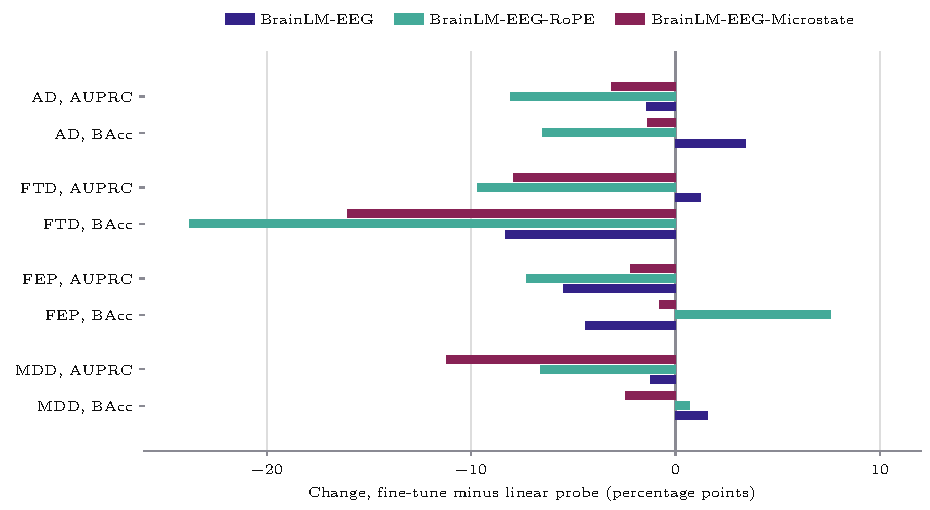
\includegraphics[width=0.9\textwidth]{figures/fig_lp_vs_ft.pdf}
\caption[Linear probing versus finetuning by task]{
Change in AUPRC and balanced accuracy after finetuning, computed as finetuned
minus linear-probed performance. Bars show the change for each proposed model,
with negative values indicating better performance under linear probing.
}
\label{fig:lp_vs_ft}
\end{figure}

The downstream evaluation pools were small, containing 52, 41, 62, and 98
participants for AD, FTD, FEP, and MDD, respectively. Compared with linear
probing, finetuning therefore updated substantially more parameters using the
same limited labelled cohorts. This is consistent with the possibility of
overfitting or unstable adaptation, but the experiment does not isolate the
cause of the observed degradation. Only the finetuning configuration
described in Section~\ref{sec:m_lp_ft} was evaluated; no per-task learning rate
search, partial unfreezing, or layer-wise learning rate schedule was compared.

Within the evaluated configuration, the more reliable use of the pretrained
encoder was therefore as a frozen representation rather than through
full-model adaptation: finetuning did not consistently improve over linear
probing under the hyperparameters and data splits used in this study. This
result does not show that finetuning is generally unsuitable for these tasks,
but it identifies linear probing as the stronger adaptation strategy in the
experiments reported here.


\section{Masking Ratio and Masking Strategy}\label{sec:r_ablation}

\begin{table}[htbp]
  \centering
  \small
  \setlength{\tabcolsep}{3pt}
  \caption[Ablation of the pretraining masking objective]{Ablation of the BrainLM-EEG pretraining objective: masking ratio (upper block, random masking) and masking strategy (lower block, 75\% masking ratio), under linear probing.}
  \label{tab:ablation_indomain}
  \resizebox{\ifdim\width>\linewidth\linewidth\else\width\fi}{!}{%
  \begin{tabular}{l cc cc cc}
    \toprule
     & \multicolumn{2}{c}{AD} & \multicolumn{2}{c}{FTD} & \multicolumn{2}{c}{FEP} \\
    \cmidrule(lr){2-3} \cmidrule(lr){4-5} \cmidrule(lr){6-7}
     & AUPRC $\uparrow$ & BAcc $\uparrow$ & AUPRC $\uparrow$ & BAcc $\uparrow$ & AUPRC $\uparrow$ & BAcc $\uparrow$ \\
    \midrule
    Random, 20\% & 86.2\,{\scriptsize$\pm$16.1} & 66.0\,{\scriptsize$\pm$9.6} & \underline{88.5\,{\scriptsize$\pm$7.1}} & 69.8\,{\scriptsize$\pm$10.9} & 62.1\,{\scriptsize$\pm$13.1} & 45.9\,{\scriptsize$\pm$5.6} \\
    Random, 50\% & 89.7\,{\scriptsize$\pm$11.5} & 74.0\,{\scriptsize$\pm$15.9} & 81.1\,{\scriptsize$\pm$6.5} & 60.5\,{\scriptsize$\pm$12.9} & 67.6\,{\scriptsize$\pm$10.7} & 45.8\,{\scriptsize$\pm$8.3} \\
    Random, 75\%$^{\star}$ & \underline{92.6\,{\scriptsize$\pm$8.0}} & \textbf{85.2\,{\scriptsize$\pm$4.0}} & 82.8\,{\scriptsize$\pm$6.5} & \underline{74.7\,{\scriptsize$\pm$14.3}} & \textbf{73.6\,{\scriptsize$\pm$15.4}} & \underline{54.8\,{\scriptsize$\pm$9.9}} \\
    Random, 90\% & \textbf{93.0\,{\scriptsize$\pm$6.6}} & \underline{83.2\,{\scriptsize$\pm$6.3}} & \textbf{91.0\,{\scriptsize$\pm$9.0}} & \textbf{75.7\,{\scriptsize$\pm$13.3}} & \underline{68.9\,{\scriptsize$\pm$6.3}} & \textbf{61.5\,{\scriptsize$\pm$4.0}} \\
    \midrule
    Random (channel $\times$ time)$^{\star}$ & \underline{92.6\,{\scriptsize$\pm$8.0}} & \underline{85.2\,{\scriptsize$\pm$4.0}} & \underline{82.8\,{\scriptsize$\pm$6.5}} & \textbf{74.7\,{\scriptsize$\pm$14.3}} & \textbf{73.6\,{\scriptsize$\pm$15.4}} & \textbf{54.8\,{\scriptsize$\pm$9.9}} \\
    Whole channels & \textbf{95.4\,{\scriptsize$\pm$4.8}} & \textbf{89.3\,{\scriptsize$\pm$8.1}} & \textbf{94.8\,{\scriptsize$\pm$6.4}} & \underline{74.0\,{\scriptsize$\pm$14.2}} & \underline{65.2\,{\scriptsize$\pm$9.5}} & \underline{53.5\,{\scriptsize$\pm$4.6}} \\
    Whole time patches & 89.5\,{\scriptsize$\pm$13.2} & 84.0\,{\scriptsize$\pm$10.9} & 81.1\,{\scriptsize$\pm$11.4} & 63.7\,{\scriptsize$\pm$14.7} & 55.7\,{\scriptsize$\pm$4.2} & 48.3\,{\scriptsize$\pm$3.4} \\
    Brain regions & 89.3\,{\scriptsize$\pm$11.4} & 82.8\,{\scriptsize$\pm$14.0} & 79.2\,{\scriptsize$\pm$3.4} & 67.3\,{\scriptsize$\pm$10.8} & 62.4\,{\scriptsize$\pm$4.7} & 52.1\,{\scriptsize$\pm$5.5} \\
    Last time patches (causal) & 91.0\,{\scriptsize$\pm$9.2} & 75.2\,{\scriptsize$\pm$13.2} & 79.4\,{\scriptsize$\pm$7.2} & 63.2\,{\scriptsize$\pm$14.2} & 52.2\,{\scriptsize$\pm$3.8} & 50.0\,{\scriptsize$\pm$0.0} \\
    \bottomrule
  \end{tabular}%
  }
  \\[3pt]
  \begin{minipage}{\linewidth}\footnotesize\raggedright
    AD: Alzheimer's disease; FTD: frontotemporal dementia; FEP: first-episode psychosis; all versus healthy controls. LP: linear probe. $^{\star}$: canonical setting (random masking, 75\%), the configuration used for BrainLM-EEG in the main tables. Best and second best are ranked within each block. Values are subject level $\times 100$. \textbf{Bold}: best per column; \underline{underline}: second best.
  \end{minipage}
\end{table}


The masking ablation examined whether downstream performance changed with the
amount and structure of masking used during BrainLM-EEG pretraining
(Section~\ref{sec:m_masking_ablation}). The analysis used the base
BrainLM-EEG model with linear probing and five-fold within-dataset evaluation.
Table~\ref{tab:ablation_indomain} reports both comparisons. MDD was not included
in this ablation because its downstream BAcc was close to chance in the preceding
evaluations.

For the masking ratio comparison, random masking was retained while the ratio
was varied. The 75\% and 90\% configurations produced higher values in five of
the six reported task metric columns. The exception was FTD AUPRC when
comparing 20\% with the canonical 75\% setting: 20\% masking achieved 88.5\%,
whereas 75\% masking achieved 82.8\%. The highest FTD AUPRC in the
masking ratio comparison was 91.0\% at 90\% masking. These results indicate
that high masking ratios did not prevent the model from learning
representations that supported the evaluated downstream tasks. They do not,
however, establish that high masking ratios are generally optimal for EEG.

% Generated by code/analysis/dataset/generate_results_figures.py.
\begin{figure}[htbp]
\centering
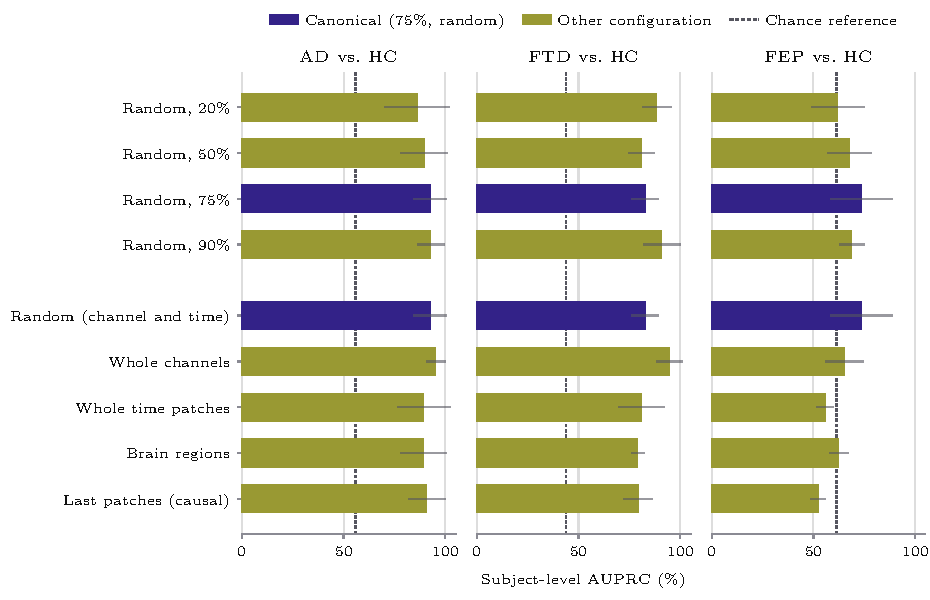
\includegraphics[width=0.9\textwidth]{figures/fig_masking_ablation.pdf}
\caption[Masking ratio and strategy ablation]{
Subject level AUPRC for masking ratio and masking strategy ablations across tasks.
The upper block varies the masking ratio under random masking; the lower block
varies the masking structure at the canonical 75\% ratio.
}
\label{fig:masking_ablation_results}
\end{figure}

For the masking strategy comparison, the masking ratio was fixed at 75\%.
Channel-wise masking produced the highest AUPRC on both neurodegenerative
tasks. On AD, it achieved 95.4\% AUPRC and 89.3\% BAcc, compared with 92.6\%
and 85.2\% for random masking. On FTD, channel-wise masking achieved 94.8\%
AUPRC compared with 82.8\% for random masking, while BAcc was similar
(74.0\% versus 74.7\%). On FEP, random masking performed better than
channel-wise masking on both reported metrics, including an AUPRC of 73.6\%
versus 65.2\%. The remaining temporal, region-wise, and forecasting style
masking strategies were below random masking in most reported columns.
Figure~\ref{fig:masking_ablation_results} summarises both ablation blocks.

The masking ablation therefore shows that the pretraining configuration matters,
but that its effect is task dependent. Channel-wise masking was favourable on
several AD and FTD comparisons, whereas random masking remained stronger on
FEP. No single masking configuration dominated all tasks and metrics. The
result is consequently not a universal best masking rule, but evidence that
the structure of the pretraining corruption changes the usefulness of the
resulting representation.


\section{Layer-Wise Representation Analysis}\label{sec:r_layers}

Having established that downstream performance depends on both task and
pretraining configuration, the layer-wise analysis asks where task relevant
information is expressed within BrainLM-EEG
(Section~\ref{sec:m_layer_probe}). Table~\ref{tab:layer_analysis_mean} reports
results based on mean-pooled patch token representations rather than the
CLS representation used in the main BrainLM-EEG analyses.

\begin{table}[htbp]
  \centering
  \small
  \setlength{\tabcolsep}{3pt}
  \caption[Layer-wise linear probe analysis]{Layer-wise linear probe analysis of BrainLM-EEG on frozen representations, pooling the mean over patch tokens (subject level).}
  \label{tab:layer_analysis_mean}
  \resizebox{\ifdim\width>\linewidth\linewidth\else\width\fi}{!}{%
  \begin{tabular}{l cc cc cc cc}
    \toprule
     & \multicolumn{2}{c}{AD} & \multicolumn{2}{c}{FTD} & \multicolumn{2}{c}{FEP} & \multicolumn{2}{c}{MDD} \\
    \cmidrule(lr){2-3} \cmidrule(lr){4-5} \cmidrule(lr){6-7} \cmidrule(lr){8-9}
     & AUPRC $\uparrow$ & BAcc $\uparrow$ & AUPRC $\uparrow$ & BAcc $\uparrow$ & AUPRC $\uparrow$ & BAcc $\uparrow$ & AUPRC $\uparrow$ & BAcc $\uparrow$ \\
    \midrule
    Layer 0 & 64.9\,{\scriptsize$\pm$14.4} & 50.0\,{\scriptsize$\pm$0.0} & 68.0\,{\scriptsize$\pm$9.7} & 50.0\,{\scriptsize$\pm$0.0} & 62.2\,{\scriptsize$\pm$14.2} & 50.0\,{\scriptsize$\pm$0.0} & \textbf{65.8\,{\scriptsize$\pm$12.3}} & \textbf{50.0\,{\scriptsize$\pm$0.0}} \\
    Layer 1 & 85.2\,{\scriptsize$\pm$10.7} & \underline{84.8\,{\scriptsize$\pm$11.0}} & \underline{90.0\,{\scriptsize$\pm$7.4}} & \textbf{78.5\,{\scriptsize$\pm$12.3}} & 65.1\,{\scriptsize$\pm$7.3} & \underline{51.8\,{\scriptsize$\pm$6.8}} & \underline{58.0\,{\scriptsize$\pm$8.2}} & \textbf{50.0\,{\scriptsize$\pm$0.0}} \\
    Layer 2 & \underline{91.9\,{\scriptsize$\pm$11.0}} & 83.3\,{\scriptsize$\pm$15.3} & \textbf{92.8\,{\scriptsize$\pm$6.8}} & \underline{70.5\,{\scriptsize$\pm$11.6}} & 68.4\,{\scriptsize$\pm$13.4} & \textbf{58.8\,{\scriptsize$\pm$11.5}} & 51.0\,{\scriptsize$\pm$7.0} & \textbf{50.0\,{\scriptsize$\pm$0.0}} \\
    Layer 3 & \textbf{95.5\,{\scriptsize$\pm$4.2}} & \textbf{87.0\,{\scriptsize$\pm$7.3}} & 86.5\,{\scriptsize$\pm$9.0} & 60.2\,{\scriptsize$\pm$9.5} & \textbf{71.0\,{\scriptsize$\pm$10.6}} & 51.1\,{\scriptsize$\pm$5.3} & 52.5\,{\scriptsize$\pm$7.4} & 48.6\,{\scriptsize$\pm$1.7} \\
    Final & 91.2\,{\scriptsize$\pm$11.7} & 78.3\,{\scriptsize$\pm$10.6} & 81.6\,{\scriptsize$\pm$14.2} & 65.5\,{\scriptsize$\pm$24.2} & \underline{68.4\,{\scriptsize$\pm$9.0}} & 50.5\,{\scriptsize$\pm$5.3} & 52.9\,{\scriptsize$\pm$6.5} & \underline{49.3\,{\scriptsize$\pm$1.4}} \\
    \bottomrule
  \end{tabular}%
  }
  \\[3pt]
  \begin{minipage}{\linewidth}\footnotesize\raggedright
    AD: Alzheimer's disease; FTD: frontotemporal dementia; FEP: first-episode psychosis; MDD: major depressive disorder; all versus healthy controls. Layer 0: patch embedding; Layers 1 to 3: transformer blocks; Final: encoder output (last block with final norm). Values are subject level $\times 100$. \textbf{Bold}: best per column; \underline{underline}: second best.
  \end{minipage}
\end{table}


For AD, layer 3 produced the strongest reported values, with 95.5\% AUPRC and
87.0\% BAcc. The final transformer layer achieved 91.2\% AUPRC and 78.3\%
BAcc, below layers 2 and 3. A similar pattern was observed for FTD, where
layer 2 achieved 92.8\% AUPRC compared with 81.6\% at the final layer. For FEP,
layers 2 and 3 also provided the strongest reported decoding performance.
Within this model and evaluation setup, task relevant decoding performance did
not consistently peak at the final transformer layer.

% Generated by code/analysis/dataset/generate_results_figures.py.
\begin{figure}[htbp]
\centering
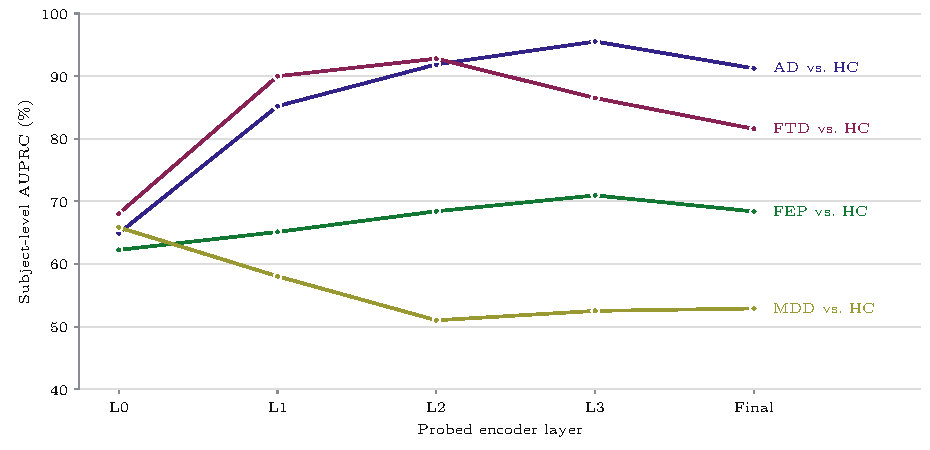
\includegraphics[width=0.8\textwidth]{figures/fig_layerwise.pdf}
\caption[Layer-wise AUPRC by depth]{
Mean-pooled patch token AUPRC across model layers for each task. AD and FTD peak
at an intermediate layer, FEP increases gradually, and MDD declines after the
patch embedding.
}
\label{fig:layerwise_results}
\end{figure}

The MDD results differed across metrics. The pre-transformer patch embedding representation, reported as layer 0, achieved 65.8\% AUPRC. AUPRC then decreased to 58.0\%, 51.0\%, 52.5\%, and 52.9\% across the transformer layers, while layer-0 BAcc was 50.0\%. This is the opposite of the pattern for AD and FTD, where the values rise sharply from layer 0 to a peak at layer 3 or layer 2 before declining slightly toward the final representation. The layer-wise results again show a difference between ranking performance and thresholded classification for MDD. No transformer layer improved on the layer-0 MDD AUPRC, but this does not imply that the representation contains no decodable MDD information, because the reported AUPRC values remain above the 26.5\% prevalence reference. Figure~\ref{fig:layerwise_results} shows these depth profiles for all four tasks.

Overall, the layer-wise analysis shows that the representation is structured
across depth rather than becoming uniformly more useful toward the encoder
output. Intermediate layers provided the highest decoding values for several
tasks, while the final layer was not consistently best. This observation is
descriptive and does not by itself identify why information changes across
encoder depth.


\section{CLS Token Contribution to Reconstruction}\label{sec:r_clstoken}

The layer-wise results concern mean-pooled patch tokens, whereas the main
BrainLM-EEG downstream analyses use the CLS token as their global
representation. Because this token has no token specific reconstruction target
during masked autoencoder pretraining, the perturbation experiment
described in Section~\ref{sec:m_cls_analysis} therefore tested whether changing
the CLS representation affected reconstruction by the decoder. The
held-out pretraining validation split contained 4,584 windows evaluated in 71
batches. For each batch, the encoder output and mask were held fixed while the
decoder was run with the original CLS token, a zero vector, or
Gaussian noise.

Perturbing the CLS token increased masked patch reconstruction MSE
in all 71 paired batches. Mean batch level MSE increased from
\(0.4492 \pm 0.0109\) with the original token to
\(0.4666 \pm 0.0110\) after zeroing the token and
\(0.4691 \pm 0.0112\) after replacement with Gaussian noise. These changes
correspond to increases of 3.86\% and 4.42\%, respectively. The one-sided
paired Wilcoxon signed-rank tests gave \(W=2556\) and
\(p=1.2\times10^{-13}\) for both perturbations at \(\alpha=0.05\). The batch level
comparison is shown in Figure~\ref{fig:cls_perturbation_results}.

% Generated by code/analysis/dataset/generate_results_figures.py. This figure is
% authored 4.2 in wide rather than at \textwidth because its axes are square;
% 0.68\textwidth reproduces it at scale 1.00, matching the other figures' type size.
\begin{figure}[htbp]
\centering
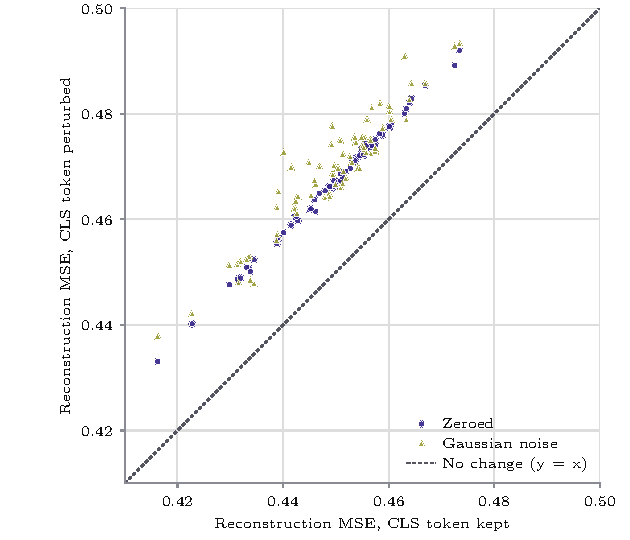
\includegraphics[width=0.68\textwidth]{figures/fig_cls_perturbation.pdf}
\caption[Reconstruction MSE under CLS perturbation]{
Masked patch reconstruction MSE with the original CLS token versus zeroed or
Gaussian-noise replacement across held-out validation batches. The dashed line
indicates equality; points above the line indicate increased MSE after
perturbation.
}
\label{fig:cls_perturbation_results}
\end{figure}

The consistent increase in reconstruction error indicates that the decoder
uses information associated with the CLS representation. However,
the experiment does not quantify what proportion of the reconstructed
information is carried by CLS, nor does it show that this token
contains clinically discriminative information. The statistical unit in this
analysis was also the batch rather than the participant. The reported
\(p\)-values therefore describe consistency across the evaluated batches and
should not be interpreted as participant level inferential evidence.


\section{Analysis of Reconstructed EEG}\label{sec:r_reconstruction}

\begin{table}[htbp]
  \centering
  \small
  \setlength{\tabcolsep}{3pt}
  \caption[BrainLM reconstruction quality assessment]{BrainLM reconstruction quality assessment: classification from the input EEG versus from the BrainLM encode$\to$decode output (subject level).}
  \label{tab:brainlm_reconstruction}
  \resizebox{\ifdim\width>\linewidth\linewidth\else\width\fi}{!}{%
  \begin{tabular}{l cc cc cc}
    \toprule
     & \multicolumn{2}{c}{AD} & \multicolumn{2}{c}{FTD} & \multicolumn{2}{c}{FEP} \\
    \cmidrule(lr){2-3} \cmidrule(lr){4-5} \cmidrule(lr){6-7}
     & AUPRC $\uparrow$ & BAcc $\uparrow$ & AUPRC $\uparrow$ & BAcc $\uparrow$ & AUPRC $\uparrow$ & BAcc $\uparrow$ \\
    \midrule
    LDA (input EEG) & 91.3\,{\scriptsize$\pm$10.9} & \textbf{94.3\,{\scriptsize$\pm$7.9}} & 77.2\,{\scriptsize$\pm$9.0} & 65.8\,{\scriptsize$\pm$11.6} & 64.4\,{\scriptsize$\pm$10.5} & 58.2\,{\scriptsize$\pm$8.3} \\
    LDA (reconstructed EEG) & \textbf{95.0\,{\scriptsize$\pm$7.1}} & 89.0\,{\scriptsize$\pm$9.0} & \textbf{89.7\,{\scriptsize$\pm$7.5}} & \textbf{81.7\,{\scriptsize$\pm$10.7}} & \textbf{72.2\,{\scriptsize$\pm$6.0}} & \textbf{65.1\,{\scriptsize$\pm$11.2}} \\
    \midrule
    ATCNet (input EEG) & 92.4\,{\scriptsize$\pm$9.5} & \textbf{83.2\,{\scriptsize$\pm$7.3}} & 87.5\,{\scriptsize$\pm$10.4} & \textbf{71.0\,{\scriptsize$\pm$25.5}} & 62.8\,{\scriptsize$\pm$5.6} & \textbf{56.5\,{\scriptsize$\pm$4.6}} \\
    ATCNet (reconstructed EEG) & \textbf{94.1\,{\scriptsize$\pm$7.8}} & 80.7\,{\scriptsize$\pm$6.1} & \textbf{89.1\,{\scriptsize$\pm$8.3}} & 65.0\,{\scriptsize$\pm$14.6} & \textbf{78.2\,{\scriptsize$\pm$5.0}} & 51.1\,{\scriptsize$\pm$6.3} \\
    \bottomrule
  \end{tabular}%
  }
  \\[3pt]
  \begin{minipage}{\linewidth}\footnotesize\raggedright
    AD: Alzheimer's disease; FTD: frontotemporal dementia; FEP: first-episode psychosis; all versus healthy controls. Reconstructed EEG is the BrainLM full-autoencoder output (mask ratio\,=\,0) of the same input, with the classifier retrained on it. Values are subject level $\times 100$. \textbf{Bold}: better of the two rows for that classifier.
  \end{minipage}
\end{table}


The final representation analysis moves from latent features back to the EEG
signal and asks whether information useful for downstream classification is
retained after reconstruction by BrainLM-EEG, following
Section~\ref{sec:m_reconstruction_analysis}. LDA and ATCNet were each trained
separately on original and reconstructed inputs for AD, FTD, and FEP.
Table~\ref{tab:brainlm_reconstruction} reports the six resulting paired
model task comparisons. MDD was not included in this analysis.

AUPRC was higher with reconstructed EEG in all six comparisons. The largest
reported increases included LDA on FTD, from 77.2\% to 89.7\% AUPRC, and
ATCNet on FEP, from 62.8\% to 78.2\% AUPRC. For LDA on FTD, BAcc also increased
from 65.8\% to 81.7\%. However, BAcc did not improve consistently. It decreased
for LDA on AD (94.3\% to 89.0\%), ATCNet on AD (83.2\% to 80.7\%), ATCNet on
FTD (71.0\% to 65.0\%), and ATCNet on FEP (56.5\% to 51.1\%), while increasing
for LDA on FTD and FEP (Figure~\ref{fig:reconstruction_asfeatures_results}).

% Generated by code/analysis/dataset/generate_results_figures.py.
\begin{figure}[htbp]
\centering
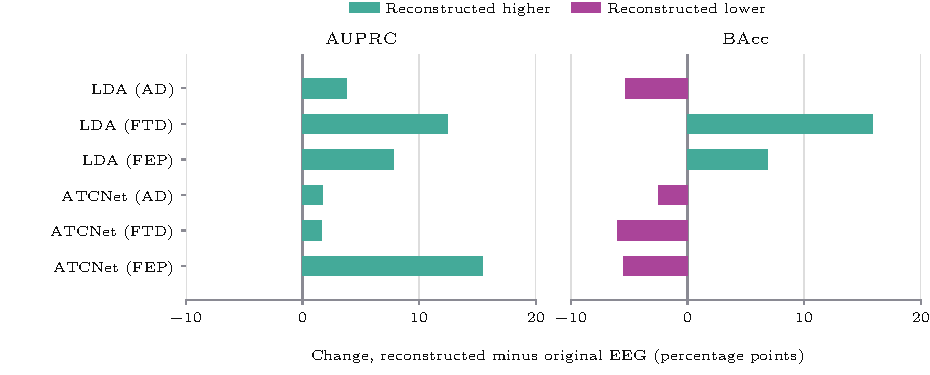
\includegraphics[width=0.85\textwidth]{figures/fig_reconstruction_asfeatures.pdf}
\caption[Original versus reconstructed EEG as classifier input]{
Change in classifier performance when using reconstructed versus original EEG
inputs. Bars show reconstructed minus original performance for AUPRC and balanced
accuracy across tasks.
}
\label{fig:reconstruction_asfeatures_results}
\end{figure}

The reconstruction experiment therefore complements the latent representation
analyses. The reconstructed inputs produced higher ranking performance in all
six reported AUPRC comparisons, while the effect on thresholded
participant level classification was mixed. This shows that the
encoder-decoder transformation retained information that the evaluated
classifiers could use, even though the experiment does not establish that
reconstruction denoises the EEG or preserves all clinically relevant
information. No inferential comparison or signal level analysis was performed,
so the finding is limited to the reported classifiers and tasks.


% \section{Summary of Findings}\label{sec:r_summary}

% The main results of this chapter can be summarised as follows. Across the four within-dataset tasks, the BrainLM-EEG variants were competitive with classical, supervised, and externally pretrained models. RoPE and Microstate improved on the base BrainLM-EEG model in several settings, particularly on AD and FTD under LOSO, but neither modification was consistently superior across tasks and metrics. No model family performed best across all tasks, and performance was sensitive to the evaluation protocol. AUPRC decreased for every model under FEP-to-SCZ transfer, highlighting the additional difficulty of cross-dataset generalisation.

% Downstream performance also varied with masking configuration, encoder depth, and adaptation strategy. Under the evaluated configuration, frozen-encoder evaluation generally outperformed full-model finetuning, while CLS-token perturbation increased reconstruction error in all 71 held-out batches and reconstructed EEG achieved higher AUPRC in all six classifier comparisons. Overall, the results show that the usefulness of the learned representations depends on the clinical task, representation design, and evaluation setting. Because the downstream model comparisons were descriptive and each pretraining configuration was run once, these results are best interpreted as broader performance patterns rather than small differences between individual models. Chapter~\ref{ch:discussion} discusses their implications.
